\begin{figure}[ht!]
  \centering
  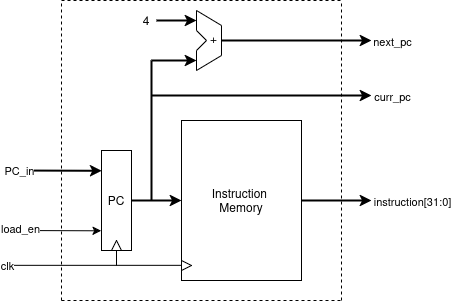
\includegraphics[scale = 0.4]{IF_BD.png}
  \caption{Basic instruction fetch block diagram}
  \label{fig:IF_BD}
\end{figure}
\section{Basic decription}
This stage of the datapath returns the necessary instruction to be executed, stored in the Instruction Memory. This can be implemented using the Block Memory Generator IP, available in the Vivado environment, as a single-port RAM with a read-write width of 32 bits and arbitrary capacity (in our case 4096 bits, making the Program Counter 12 bits of length).
The Program Counter (PC) holds the address of the current instruction. While a program is running, it will be incremented by default by 4 to fetch the next address, as instructions are word-aligned and 32 bits wide. In order to manage jumps between various segments of a program, another value can be loaded from another stage after the instruction is decoded and executed.
In VHDL, a register can be synthesized by declaring a clock-dependent (and in this case also \emph{load{\_}en} dependent) \emph{signal}, hence the PC will be implemented with this method.
A VHDL entity that describes this stage can be defined as follows:\\
\begin{minted}[fontsize=\footnotesize]{vhdl}
entity instr_fetch is
 port ( 
  clk        : in std_logic;
  pc_load_en : in std_logic;
  pc_in      : in std_logic_vector(11 downto 0);
       
  next_pc    : out std_logic_vector(11 downto 0);
  curr_pc    : out std_logic_vector(11 downto 0);
  instr      : out std_logic_vector(31 downto 0)
  );
end instr_fetch;
\end{minted}
\vspace{1\baselineskip}
With the previously specified settings, the IP used for the Instruction Memory will generate a component that can be instantiated in the architecture as follows:\\
\begin{minted}[fontsize=\footnotesize]{vhdl}
component instruction_memory
 port(
  clka  : in std_logic;
  wea   : in std_logic;
  addra : in std_logic_vector(9 downto 0);
  dina  : in std_logic_vector(31 downto 0);
  douta : out std_logic_vector(31 downto 0));
end component;
\end{minted}
\vspace{1\baselineskip}
The inputs \emph{wea} (i.e. the write-enabling input) and \emph{dina} (data input for port A) will be pulled low since there is no need for the moment to write inside the memory. 
Since the PC has to act as a pointer for the instruction, its output will be routed to the \emph{addra} input, excluding the first two least significant bits in order to proceed 32 bits (the length of a standard instruction) at a time.
With this being said, the only thing that is left to do is a clock-sensitive process that increments the PC or loads another address from the outside if the load-enable input of its register is pulled high. 
By implementing the register as a \emph{signal} named \emph{pc{\_}reg}, the resulting VHDL script for the architecture is the following:\\
\begin{minted}[fontsize=\footnotesize]{vhdl}
architecture Structural of instr_fetch is
  signal pc_reg  : unsigned(11 downto 0) := (others => '0');

  component instruction_memory
  port(
      clka        : in std_logic;
      wea         : in std_logic;
      addra       : in std_logic_vector(9 downto 0);
      dina        : in std_logic_vector(31 downto 0);
      douta       : out std_logic_vector(31 downto 0)
  );
  end component;
begin
  instr_mem: instruction_memory 
  port map(
      clka        => clk,
      wea         => '0',
      dina        => (others => '0'),
      addra       => std_logic_vector(pc_reg(11 downto 2)),
      douta       => instr
  );
  
  process (clk)
  begin
      if rising_edge(clk) then
          if pc_load_en = '1' then
              pc_reg  <= unsigned(pc_in);
          end if;
      end if;
  end process;
  next_pc     <= std_logic_vector(pc_reg + 4);
  curr_pc     <= std_logic_vector(pc_reg);
end Structural;
\end{minted}

\section{Simulation}
A testbench for this simulation will require the PC to be incremented by 4 so that every location in the memory is addressed, but in order to actually see a stream of instructions at the output a .coe file for the initialization of the instruction memory is required:

\begin{minted}{text}
  memory_initialization_radix=16;
  memory_initialization_vector=
  00000293,                         % addi x5, x0, 0
  00100313,                         % addi x6, x0, 1
  005303B3;                         % add x7, x6, x5
\end{minted}
A .coe file requires the hexadecimal dump of the program, in this given example each instruction has its assembly equivalent on the right.\\
For the testbench, a simple clock can be simulated with a process while a small register can be simulated for storing \emph{next{\_}pc} and re-routing its value on \emph{pc{\_}in}, hence the following testbench with the resulting simulation:

\begin{minted}[fontsize=\footnotesize]{vhdl}
architecture Behavioral of IF_testbench is
  constant clk_period     : time := 20 ns;
  signal pc_in            : std_logic_vector(11 downto 0) := (others => '0');
  signal next_pc          : std_logic_vector(11 downto 0) := (others => '0');
  signal curr_pc          : std_logic_vector(11 downto 0) := (others => '0');
  signal instr            : std_logic_vector(31 downto 0) := (others => '0');
  signal clk              : std_logic := '0';
  signal pc_load_en       : std_logic := '1';
  
  component instr_fetch
      port ( 
          clk             : in std_logic;
          pc_load_en      : in std_logic;
          pc_in           : in std_logic_vector(11 downto 0);
          
          next_pc         : out std_logic_vector(11 downto 0);
          curr_pc         : out std_logic_vector(11 downto 0);
          instr           : out std_logic_vector(31 downto 0)
      );
  end component;

begin

  if_inst : instr_fetch
      port map (
          clk         => clk,
          pc_load_en  => pc_load_en,
          pc_in       => pc_in,
          next_pc     => next_pc,
          curr_pc     => curr_pc,
          instr       => instr
      );

  process
  begin
      clk <= '0';
      wait for clk_period / 2;
      clk <= '1';
      wait for clk_period / 2;
  end process;

  pc_in       <= next_pc_reg;
end Behavioral;
\end{minted}

\begin{figure}[h!]
  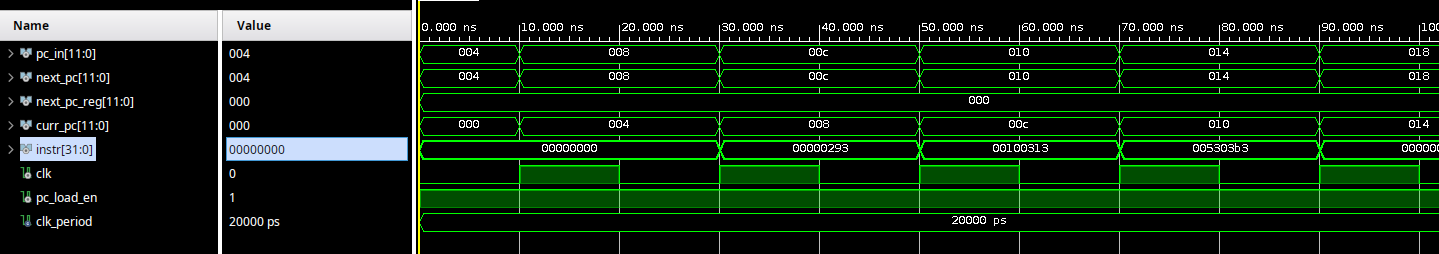
\includegraphics[scale = 0.313]{IF_sim.png}
\end{figure}

The results from the simulations state that \emph{curr{\_}pc}, in fact, acts as a register, refreshed as the clock's rising edge approaches, and the flow of instructions are the same as the ones stated in the \emph{.coe} file. 
\let\cleardoublepage\clearpage